\documentclass{standalone}
\usepackage{tikz}
\usetikzlibrary{patterns, positioning}

\begin{document}
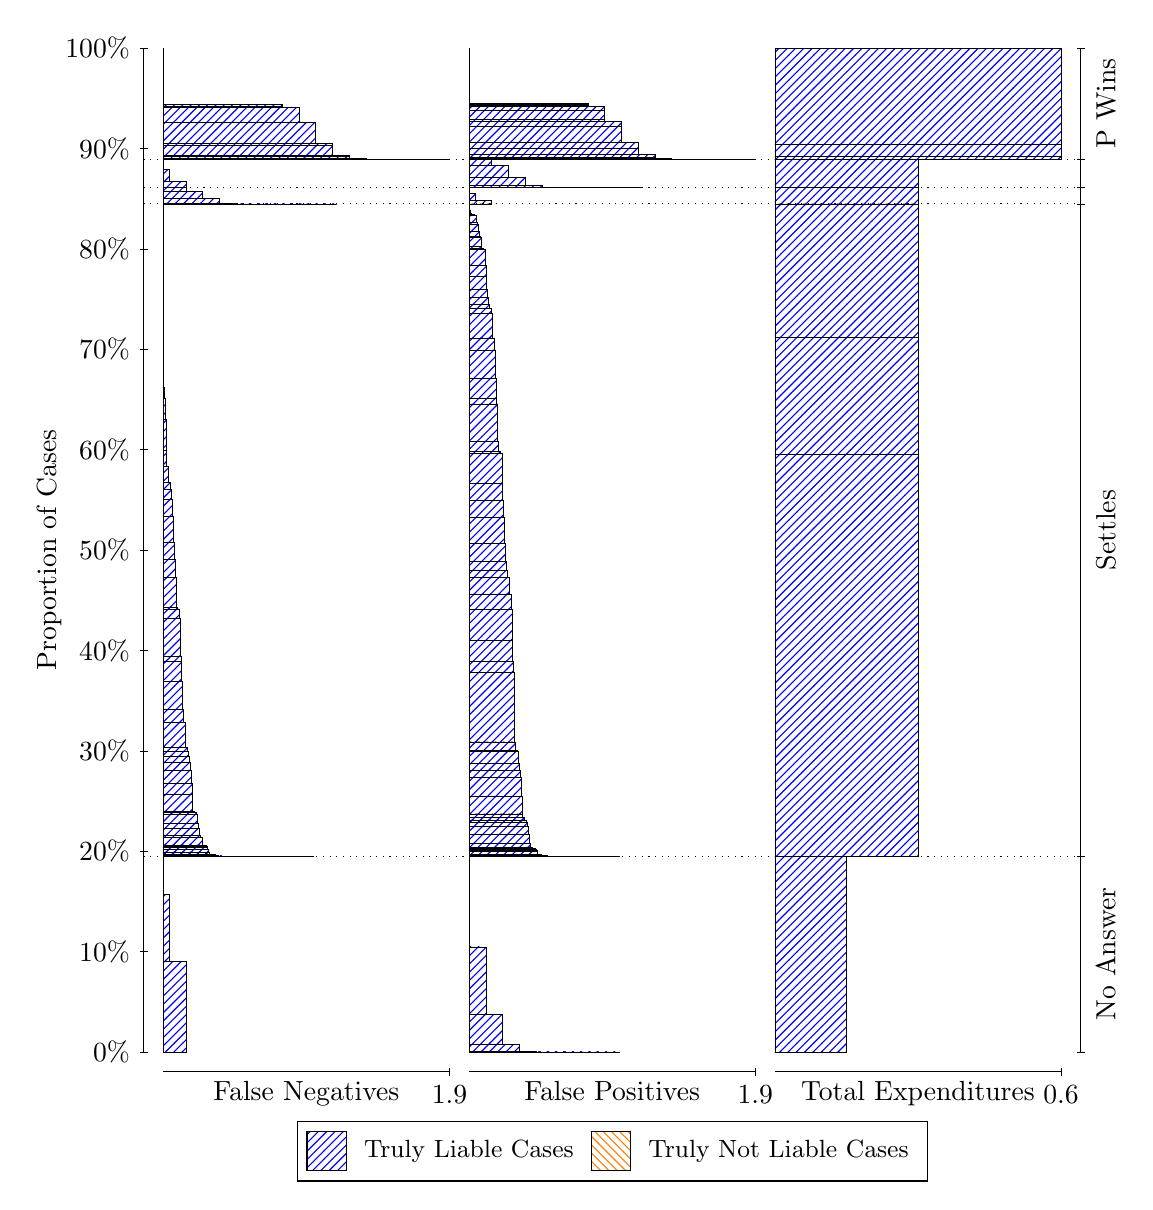
\begin{tikzpicture}
\draw[black, very thin] (1.5,1.75) -- (1.5,14.5);
\node[rotate=90, anchor=center] at (0.3, 8.125) {Proportion of Cases};
\draw[black, very thin] (1.45,1.75) -- (1.55,1.75);
\node[anchor=east] at (1.45, 1.75) {0\%};
\draw[black, very thin] (1.45,3.025) -- (1.55,3.025);
\node[anchor=east] at (1.45, 3.025) {10\%};
\draw[black, very thin] (1.45,4.3) -- (1.55,4.3);
\node[anchor=east] at (1.45, 4.3) {20\%};
\draw[black, very thin] (1.45,5.575) -- (1.55,5.575);
\node[anchor=east] at (1.45, 5.575) {30\%};
\draw[black, very thin] (1.45,6.85) -- (1.55,6.85);
\node[anchor=east] at (1.45, 6.85) {40\%};
\draw[black, very thin] (1.45,8.125) -- (1.55,8.125);
\node[anchor=east] at (1.45, 8.125) {50\%};
\draw[black, very thin] (1.45,9.4) -- (1.55,9.4);
\node[anchor=east] at (1.45, 9.4) {60\%};
\draw[black, very thin] (1.45,10.675) -- (1.55,10.675);
\node[anchor=east] at (1.45, 10.675) {70\%};
\draw[black, very thin] (1.45,11.95) -- (1.55,11.95);
\node[anchor=east] at (1.45, 11.95) {80\%};
\draw[black, very thin] (1.45,13.225) -- (1.55,13.225);
\node[anchor=east] at (1.45, 13.225) {90\%};
\draw[black, very thin] (1.45,14.5) -- (1.55,14.5);
\node[anchor=east] at (1.45, 14.5) {100\%};

\draw[black, very thin] (13.4,1.75) -- (13.4,14.5);
\draw[black, very thin] (13.35,1.75) -- (13.45,1.75);
\node[anchor=west] at (13.35, 1.75) {};
\draw[black, very thin] (13.35,4.2363) -- (13.45,4.2363);
\node[anchor=west] at (13.35, 4.2363) {};
\draw[black, very thin] (13.35,12.521) -- (13.45,12.521);
\node[anchor=west] at (13.35, 12.521) {};
\draw[black, very thin] (13.35,12.727) -- (13.45,12.727);
\node[anchor=west] at (13.35, 12.727) {};
\draw[black, very thin] (13.35,13.085) -- (13.45,13.085);
\node[anchor=west] at (13.35, 13.085) {};
\draw[black, very thin] (13.35,14.5) -- (13.45,14.5);
\node[anchor=west] at (13.35, 14.5) {};

\draw[black, very thin, pattern color=blue, pattern=north east lines] (1.75,1.75) rectangle (2.0368,2.9018);
\draw[black, very thin, pattern color=blue, pattern=north east lines] (1.75,2.9018) rectangle (1.8244,3.7553);
\draw[black, very thin, pattern color=orange, pattern=north west lines] (1.75,3.7553) rectangle (1.75,3.7553);
\draw[black, very thin, pattern color=blue, pattern=north east lines] (1.75,3.7553) rectangle (1.75,4.2363);
\draw[black, very thin, pattern color=blue, pattern=north east lines] (1.75,4.2363) rectangle (3.6623,4.2363);
\draw[black, very thin, pattern color=blue, pattern=north east lines] (1.75,4.2363) rectangle (3.5667,4.2363);
\draw[black, very thin, pattern color=blue, pattern=north east lines] (1.75,4.2363) rectangle (3.4711,4.2363);
\draw[black, very thin, pattern color=blue, pattern=north east lines] (1.75,4.2363) rectangle (3.4498,4.2363);
\draw[black, very thin, pattern color=blue, pattern=north east lines] (1.75,4.2363) rectangle (3.3754,4.2363);
\draw[black, very thin, pattern color=blue, pattern=north east lines] (1.75,4.2363) rectangle (3.3542,4.2363);
\draw[black, very thin, pattern color=blue, pattern=north east lines] (1.75,4.2363) rectangle (3.2798,4.2363);
\draw[black, very thin, pattern color=blue, pattern=north east lines] (1.75,4.2363) rectangle (3.2586,4.2363);
\draw[black, very thin, pattern color=blue, pattern=north east lines] (1.75,4.2363) rectangle (3.2373,4.2363);
\draw[black, very thin, pattern color=blue, pattern=north east lines] (1.75,4.2363) rectangle (3.1842,4.2363);
\draw[black, very thin, pattern color=blue, pattern=north east lines] (1.75,4.2363) rectangle (3.163,4.2363);
\draw[black, very thin, pattern color=blue, pattern=north east lines] (1.75,4.2363) rectangle (3.1417,4.2363);
\draw[black, very thin, pattern color=blue, pattern=north east lines] (1.75,4.2363) rectangle (3.0886,4.2363);
\draw[black, very thin, pattern color=blue, pattern=north east lines] (1.75,4.2363) rectangle (3.0673,4.2363);
\draw[black, very thin, pattern color=blue, pattern=north east lines] (1.75,4.2363) rectangle (3.0461,4.2363);
\draw[black, very thin, pattern color=blue, pattern=north east lines] (1.75,4.2363) rectangle (3.0249,4.2363);
\draw[black, very thin, pattern color=blue, pattern=north east lines] (1.75,4.2363) rectangle (2.993,4.2363);
\draw[black, very thin, pattern color=blue, pattern=north east lines] (1.75,4.2363) rectangle (2.9717,4.2363);
\draw[black, very thin, pattern color=blue, pattern=north east lines] (1.75,4.2363) rectangle (2.9505,4.2363);
\draw[black, very thin, pattern color=blue, pattern=north east lines] (1.75,4.2363) rectangle (2.9292,4.2363);
\draw[black, very thin, pattern color=blue, pattern=north east lines] (1.75,4.2363) rectangle (2.8974,4.2363);
\draw[black, very thin, pattern color=blue, pattern=north east lines] (1.75,4.2363) rectangle (2.8761,4.2363);
\draw[black, very thin, pattern color=blue, pattern=north east lines] (1.75,4.2363) rectangle (2.8549,4.2363);
\draw[black, very thin, pattern color=blue, pattern=north east lines] (1.75,4.2363) rectangle (2.8336,4.2363);
\draw[black, very thin, pattern color=blue, pattern=north east lines] (1.75,4.2363) rectangle (2.8124,4.2363);
\draw[black, very thin, pattern color=blue, pattern=north east lines] (1.75,4.2363) rectangle (2.8018,4.2363);
\draw[black, very thin, pattern color=blue, pattern=north east lines] (1.75,4.2363) rectangle (2.7805,4.2363);
\draw[black, very thin, pattern color=blue, pattern=north east lines] (1.75,4.2363) rectangle (2.7593,4.2363);
\draw[black, very thin, pattern color=blue, pattern=north east lines] (1.75,4.2363) rectangle (2.738,4.2363);
\draw[black, very thin, pattern color=blue, pattern=north east lines] (1.75,4.2363) rectangle (2.7168,4.2363);
\draw[black, very thin, pattern color=blue, pattern=north east lines] (1.75,4.2363) rectangle (2.7061,4.2363);
\draw[black, very thin, pattern color=blue, pattern=north east lines] (1.75,4.2363) rectangle (2.6849,4.2363);
\draw[black, very thin, pattern color=blue, pattern=north east lines] (1.75,4.2363) rectangle (2.6636,4.2364);
\draw[black, very thin, pattern color=blue, pattern=north east lines] (1.75,4.2364) rectangle (2.6424,4.2364);
\draw[black, very thin, pattern color=blue, pattern=north east lines] (1.75,4.2364) rectangle (2.6212,4.2364);
\draw[black, very thin, pattern color=blue, pattern=north east lines] (1.75,4.2364) rectangle (2.6105,4.2364);
\draw[black, very thin, pattern color=blue, pattern=north east lines] (1.75,4.2364) rectangle (2.5999,4.2366);
\draw[black, very thin, pattern color=blue, pattern=north east lines] (1.75,4.2366) rectangle (2.5893,4.2366);
\draw[black, very thin, pattern color=blue, pattern=north east lines] (1.75,4.2366) rectangle (2.568,4.2366);
\draw[black, very thin, pattern color=blue, pattern=north east lines] (1.75,4.2366) rectangle (2.5468,4.2371);
\draw[black, very thin, pattern color=blue, pattern=north east lines] (1.75,4.2371) rectangle (2.5255,4.2385);
\draw[black, very thin, pattern color=blue, pattern=north east lines] (1.75,4.2385) rectangle (2.5149,4.2387);
\draw[black, very thin, pattern color=blue, pattern=north east lines] (1.75,4.2387) rectangle (2.5043,4.2389);
\draw[black, very thin, pattern color=blue, pattern=north east lines] (1.75,4.2389) rectangle (2.4937,4.239);
\draw[black, very thin, pattern color=blue, pattern=north east lines] (1.75,4.239) rectangle (2.4724,4.2391);
\draw[black, very thin, pattern color=blue, pattern=north east lines] (1.75,4.2391) rectangle (2.4512,4.2443);
\draw[black, very thin, pattern color=blue, pattern=north east lines] (1.75,4.2443) rectangle (2.4299,4.245);
\draw[black, very thin, pattern color=blue, pattern=north east lines] (1.75,4.245) rectangle (2.4193,4.2523);
\draw[black, very thin, pattern color=blue, pattern=north east lines] (1.75,4.2523) rectangle (2.4087,4.2554);
\draw[black, very thin, pattern color=blue, pattern=north east lines] (1.75,4.2554) rectangle (2.3981,4.2555);
\draw[black, very thin, pattern color=blue, pattern=north east lines] (1.75,4.2555) rectangle (2.3874,4.2646);
\draw[black, very thin, pattern color=blue, pattern=north east lines] (1.75,4.2646) rectangle (2.3768,4.2655);
\draw[black, very thin, pattern color=blue, pattern=north east lines] (1.75,4.2655) rectangle (2.3556,4.2661);
\draw[black, very thin, pattern color=blue, pattern=north east lines] (1.75,4.2661) rectangle (2.3343,4.2907);
\draw[black, very thin, pattern color=blue, pattern=north east lines] (1.75,4.2907) rectangle (2.3237,4.3204);
\draw[black, very thin, pattern color=blue, pattern=north east lines] (1.75,4.3204) rectangle (2.3131,4.3527);
\draw[black, very thin, pattern color=blue, pattern=north east lines] (1.75,4.3527) rectangle (2.3024,4.3599);
\draw[black, very thin, pattern color=blue, pattern=north east lines] (1.75,4.3599) rectangle (2.2918,4.3688);
\draw[black, very thin, pattern color=blue, pattern=north east lines] (1.75,4.3688) rectangle (2.2812,4.3742);
\draw[black, very thin, pattern color=blue, pattern=north east lines] (1.75,4.3742) rectangle (2.2599,4.3809);
\draw[black, very thin, pattern color=blue, pattern=north east lines] (1.75,4.3809) rectangle (2.2387,4.4757);
\draw[black, very thin, pattern color=blue, pattern=north east lines] (1.75,4.4757) rectangle (2.2174,4.5001);
\draw[black, very thin, pattern color=blue, pattern=north east lines] (1.75,4.5001) rectangle (2.2068,4.5868);
\draw[black, very thin, pattern color=blue, pattern=north east lines] (1.75,4.5868) rectangle (2.1962,4.649);
\draw[black, very thin, pattern color=blue, pattern=north east lines] (1.75,4.649) rectangle (2.1856,4.6552);
\draw[black, very thin, pattern color=blue, pattern=north east lines] (1.75,4.6552) rectangle (2.175,4.7739);
\draw[black, very thin, pattern color=blue, pattern=north east lines] (1.75,4.7739) rectangle (2.1643,4.7983);
\draw[black, very thin, pattern color=blue, pattern=north east lines] (1.75,4.7983) rectangle (2.1431,4.8073);
\draw[black, very thin, pattern color=blue, pattern=north east lines] (1.75,4.8073) rectangle (2.1218,5.02);
\draw[black, very thin, pattern color=blue, pattern=north east lines] (1.75,5.02) rectangle (2.1112,5.16);
\draw[black, very thin, pattern color=blue, pattern=north east lines] (1.75,5.16) rectangle (2.1006,5.327);
\draw[black, very thin, pattern color=blue, pattern=north east lines] (1.75,5.327) rectangle (2.09,5.4236);
\draw[black, very thin, pattern color=blue, pattern=north east lines] (1.75,5.4236) rectangle (2.0793,5.5097);
\draw[black, very thin, pattern color=blue, pattern=north east lines] (1.75,5.5097) rectangle (2.0687,5.5675);
\draw[black, very thin, pattern color=blue, pattern=north east lines] (1.75,5.5675) rectangle (2.0475,5.6242);
\draw[black, very thin, pattern color=blue, pattern=north east lines] (1.75,5.6242) rectangle (2.0262,5.9394);
\draw[black, very thin, pattern color=blue, pattern=north east lines] (1.75,5.9394) rectangle (2.005,6.0992);
\draw[black, very thin, pattern color=blue, pattern=north east lines] (1.75,6.0992) rectangle (1.9943,6.4537);
\draw[black, very thin, pattern color=blue, pattern=north east lines] (1.75,6.4537) rectangle (1.9837,6.7109);
\draw[black, very thin, pattern color=blue, pattern=north east lines] (1.75,6.7109) rectangle (1.9731,6.7782);
\draw[black, very thin, pattern color=blue, pattern=north east lines] (1.75,6.7782) rectangle (1.9625,7.2541);
\draw[black, very thin, pattern color=blue, pattern=north east lines] (1.75,7.2541) rectangle (1.9519,7.3782);
\draw[black, very thin, pattern color=blue, pattern=north east lines] (1.75,7.3782) rectangle (1.9306,7.4026);
\draw[black, very thin, pattern color=blue, pattern=north east lines] (1.75,7.4026) rectangle (1.9094,7.7796);
\draw[black, very thin, pattern color=blue, pattern=north east lines] (1.75,7.7796) rectangle (1.8987,8.004);
\draw[black, very thin, pattern color=blue, pattern=north east lines] (1.75,8.004) rectangle (1.8881,8.222);
\draw[black, very thin, pattern color=blue, pattern=north east lines] (1.75,8.222) rectangle (1.8775,8.5508);
\draw[black, very thin, pattern color=blue, pattern=north east lines] (1.75,8.5508) rectangle (1.8669,8.773);
\draw[black, very thin, pattern color=blue, pattern=north east lines] (1.75,8.773) rectangle (1.8562,8.8899);
\draw[black, very thin, pattern color=blue, pattern=north east lines] (1.75,8.8899) rectangle (1.835,8.9849);
\draw[black, very thin, pattern color=blue, pattern=north east lines] (1.75,8.9849) rectangle (1.8137,9.1899);
\draw[black, very thin, pattern color=blue, pattern=north east lines] (1.75,9.1899) rectangle (1.7925,9.3871);
\draw[black, very thin, pattern color=blue, pattern=north east lines] (1.75,9.3871) rectangle (1.7819,9.7801);
\draw[black, very thin, pattern color=blue, pattern=north east lines] (1.75,9.7801) rectangle (1.7712,10.051);
\draw[black, very thin, pattern color=blue, pattern=north east lines] (1.75,10.051) rectangle (1.7606,10.189);
\draw[black, very thin, pattern color=orange, pattern=north west lines] (1.75,10.189) rectangle (1.75,10.189);
\draw[black, very thin, pattern color=blue, pattern=north east lines] (1.75,10.189) rectangle (1.75,12.521);
\draw[black, very thin, pattern color=blue, pattern=north east lines] (1.75,12.521) rectangle (3.9491,12.521);
\draw[black, very thin, pattern color=blue, pattern=north east lines] (1.75,12.521) rectangle (3.7366,12.521);
\draw[black, very thin, pattern color=blue, pattern=north east lines] (1.75,12.521) rectangle (3.5242,12.521);
\draw[black, very thin, pattern color=blue, pattern=north east lines] (1.75,12.521) rectangle (3.3117,12.521);
\draw[black, very thin, pattern color=blue, pattern=north east lines] (1.75,12.521) rectangle (3.0992,12.521);
\draw[black, very thin, pattern color=blue, pattern=north east lines] (1.75,12.521) rectangle (2.8867,12.522);
\draw[black, very thin, pattern color=blue, pattern=north east lines] (1.75,12.522) rectangle (2.6743,12.53);
\draw[black, very thin, pattern color=blue, pattern=north east lines] (1.75,12.53) rectangle (2.4618,12.592);
\draw[black, very thin, pattern color=blue, pattern=north east lines] (1.75,12.592) rectangle (2.2493,12.684);
\draw[black, very thin, pattern color=blue, pattern=north east lines] (1.75,12.684) rectangle (2.0368,12.727);
\draw[black, very thin, pattern color=orange, pattern=north west lines] (1.75,12.727) rectangle (1.75,12.727);
\draw[black, very thin, pattern color=blue, pattern=north east lines] (1.75,12.727) rectangle (2.0368,12.806);
\draw[black, very thin, pattern color=blue, pattern=north east lines] (1.75,12.806) rectangle (1.8244,12.957);
\draw[black, very thin, pattern color=orange, pattern=north west lines] (1.75,12.957) rectangle (1.75,12.957);
\draw[black, very thin, pattern color=blue, pattern=north east lines] (1.75,12.957) rectangle (1.75,13.085);
\draw[black, very thin, pattern color=blue, pattern=north east lines] (1.75,13.085) rectangle (5.3833,13.085);
\draw[black, very thin, pattern color=blue, pattern=north east lines] (1.75,13.085) rectangle (5.1709,13.085);
\draw[black, very thin, pattern color=blue, pattern=north east lines] (1.75,13.085) rectangle (4.9584,13.085);
\draw[black, very thin, pattern color=blue, pattern=north east lines] (1.75,13.085) rectangle (4.7459,13.085);
\draw[black, very thin, pattern color=blue, pattern=north east lines] (1.75,13.085) rectangle (4.7459,13.085);
\draw[black, very thin, pattern color=blue, pattern=north east lines] (1.75,13.085) rectangle (4.5334,13.086);
\draw[black, very thin, pattern color=blue, pattern=north east lines] (1.75,13.086) rectangle (4.5334,13.086);
\draw[black, very thin, pattern color=blue, pattern=north east lines] (1.75,13.086) rectangle (4.321,13.087);
\draw[black, very thin, pattern color=blue, pattern=north east lines] (1.75,13.087) rectangle (4.321,13.095);
\draw[black, very thin, pattern color=blue, pattern=north east lines] (1.75,13.095) rectangle (4.1085,13.119);
\draw[black, very thin, pattern color=blue, pattern=north east lines] (1.75,13.119) rectangle (4.1085,13.14);
\draw[black, very thin, pattern color=blue, pattern=north east lines] (1.75,13.14) rectangle (3.896,13.267);
\draw[black, very thin, pattern color=blue, pattern=north east lines] (1.75,13.267) rectangle (3.896,13.29);
\draw[black, very thin, pattern color=blue, pattern=north east lines] (1.75,13.29) rectangle (3.6835,13.558);
\draw[black, very thin, pattern color=blue, pattern=north east lines] (1.75,13.558) rectangle (3.4711,13.75);
\draw[black, very thin, pattern color=blue, pattern=north east lines] (1.75,13.75) rectangle (3.2586,13.76);
\draw[black, very thin, pattern color=blue, pattern=north east lines] (1.75,13.76) rectangle (3.2586,13.785);
\draw[black, very thin, pattern color=blue, pattern=north east lines] (1.75,13.785) rectangle (3.0461,13.785);
\draw[black, very thin, pattern color=blue, pattern=north east lines] (1.75,13.785) rectangle (3.0461,13.786);
\draw[black, very thin, pattern color=blue, pattern=north east lines] (1.75,13.786) rectangle (3.0461,13.786);
\draw[black, very thin, pattern color=blue, pattern=north east lines] (1.75,13.786) rectangle (2.8336,13.786);
\draw[black, very thin, pattern color=blue, pattern=north east lines] (1.75,13.786) rectangle (2.8336,13.786);
\draw[black, very thin, pattern color=blue, pattern=north east lines] (1.75,13.786) rectangle (2.6636,13.786);
\draw[black, very thin, pattern color=blue, pattern=north east lines] (1.75,13.786) rectangle (2.6212,13.786);
\draw[black, very thin, pattern color=blue, pattern=north east lines] (1.75,13.786) rectangle (2.6212,13.786);
\draw[black, very thin, pattern color=blue, pattern=north east lines] (1.75,13.786) rectangle (2.4512,13.786);
\draw[black, very thin, pattern color=blue, pattern=north east lines] (1.75,13.786) rectangle (2.4087,13.786);
\draw[black, very thin, pattern color=blue, pattern=north east lines] (1.75,13.786) rectangle (2.4087,13.786);
\draw[black, very thin, pattern color=blue, pattern=north east lines] (1.75,13.786) rectangle (2.2387,13.786);
\draw[black, very thin, pattern color=blue, pattern=north east lines] (1.75,13.786) rectangle (2.2387,13.786);
\draw[black, very thin, pattern color=blue, pattern=north east lines] (1.75,13.786) rectangle (2.1962,13.786);
\draw[black, very thin, pattern color=blue, pattern=north east lines] (1.75,13.786) rectangle (2.1962,13.786);
\draw[black, very thin, pattern color=blue, pattern=north east lines] (1.75,13.786) rectangle (2.0262,13.786);
\draw[black, very thin, pattern color=blue, pattern=north east lines] (1.75,13.786) rectangle (2.0262,13.786);
\draw[black, very thin, pattern color=blue, pattern=north east lines] (1.75,13.786) rectangle (1.9837,13.786);
\draw[black, very thin, pattern color=blue, pattern=north east lines] (1.75,13.786) rectangle (1.8137,13.786);
\draw[black, very thin, pattern color=blue, pattern=north east lines] (1.75,13.786) rectangle (1.8137,13.786);
\draw[black, very thin, pattern color=blue, pattern=north east lines] (1.75,13.786) rectangle (1.8137,13.786);
\draw[black, very thin, pattern color=orange, pattern=north west lines] (1.75,13.786) rectangle (1.75,13.786);
\draw[black, very thin, pattern color=blue, pattern=north east lines] (1.75,13.786) rectangle (1.75,14.5);
\draw[black, very thin, pattern color=orange, pattern=north west lines] (5.6333,1.75) rectangle (7.5456,1.75);
\draw[black, very thin, pattern color=blue, pattern=north east lines] (5.6333,1.75) rectangle (7.5456,1.75);
\draw[black, very thin, pattern color=blue, pattern=north east lines] (5.6333,1.75) rectangle (7.3331,1.75);
\draw[black, very thin, pattern color=blue, pattern=north east lines] (5.6333,1.75) rectangle (7.1207,1.75);
\draw[black, very thin, pattern color=blue, pattern=north east lines] (5.6333,1.75) rectangle (6.9082,1.75);
\draw[black, very thin, pattern color=blue, pattern=north east lines] (5.6333,1.75) rectangle (6.6957,1.7503);
\draw[black, very thin, pattern color=blue, pattern=north east lines] (5.6333,1.7503) rectangle (6.4832,1.7582);
\draw[black, very thin, pattern color=blue, pattern=north east lines] (5.6333,1.7582) rectangle (6.2708,1.8431);
\draw[black, very thin, pattern color=blue, pattern=north east lines] (5.6333,1.8431) rectangle (6.0583,2.231);
\draw[black, very thin, pattern color=blue, pattern=north east lines] (5.6333,2.231) rectangle (5.8458,3.0845);
\draw[black, very thin, pattern color=blue, pattern=north east lines] (5.6333,3.0845) rectangle (5.6333,4.2363);
\draw[black, very thin, pattern color=orange, pattern=north west lines] (5.6333,4.2363) rectangle (7.5456,4.2363);
\draw[black, very thin, pattern color=blue, pattern=north east lines] (5.6333,4.2363) rectangle (7.5456,4.2363);
\draw[black, very thin, pattern color=orange, pattern=north west lines] (5.6333,4.2363) rectangle (7.45,4.2363);
\draw[black, very thin, pattern color=blue, pattern=north east lines] (5.6333,4.2363) rectangle (7.45,4.2363);
\draw[black, very thin, pattern color=orange, pattern=north west lines] (5.6333,4.2363) rectangle (7.3544,4.2363);
\draw[black, very thin, pattern color=blue, pattern=north east lines] (5.6333,4.2363) rectangle (7.3544,4.2363);
\draw[black, very thin, pattern color=blue, pattern=north east lines] (5.6333,4.2363) rectangle (7.3331,4.2363);
\draw[black, very thin, pattern color=orange, pattern=north west lines] (5.6333,4.2363) rectangle (7.2588,4.2363);
\draw[black, very thin, pattern color=blue, pattern=north east lines] (5.6333,4.2363) rectangle (7.2588,4.2363);
\draw[black, very thin, pattern color=blue, pattern=north east lines] (5.6333,4.2363) rectangle (7.2375,4.2363);
\draw[black, very thin, pattern color=orange, pattern=north west lines] (5.6333,4.2363) rectangle (7.1632,4.2363);
\draw[black, very thin, pattern color=blue, pattern=north east lines] (5.6333,4.2363) rectangle (7.1632,4.2363);
\draw[black, very thin, pattern color=blue, pattern=north east lines] (5.6333,4.2363) rectangle (7.1419,4.2363);
\draw[black, very thin, pattern color=blue, pattern=north east lines] (5.6333,4.2363) rectangle (7.1207,4.2363);
\draw[black, very thin, pattern color=orange, pattern=north west lines] (5.6333,4.2363) rectangle (7.0675,4.2363);
\draw[black, very thin, pattern color=blue, pattern=north east lines] (5.6333,4.2363) rectangle (7.0675,4.2363);
\draw[black, very thin, pattern color=blue, pattern=north east lines] (5.6333,4.2363) rectangle (7.0463,4.2363);
\draw[black, very thin, pattern color=blue, pattern=north east lines] (5.6333,4.2363) rectangle (7.025,4.2363);
\draw[black, very thin, pattern color=orange, pattern=north west lines] (5.6333,4.2363) rectangle (6.9719,4.2363);
\draw[black, very thin, pattern color=blue, pattern=north east lines] (5.6333,4.2363) rectangle (6.9719,4.2363);
\draw[black, very thin, pattern color=blue, pattern=north east lines] (5.6333,4.2363) rectangle (6.9507,4.2363);
\draw[black, very thin, pattern color=blue, pattern=north east lines] (5.6333,4.2363) rectangle (6.9294,4.2363);
\draw[black, very thin, pattern color=blue, pattern=north east lines] (5.6333,4.2363) rectangle (6.9082,4.2363);
\draw[black, very thin, pattern color=orange, pattern=north west lines] (5.6333,4.2363) rectangle (6.8763,4.2363);
\draw[black, very thin, pattern color=blue, pattern=north east lines] (5.6333,4.2363) rectangle (6.8763,4.2363);
\draw[black, very thin, pattern color=blue, pattern=north east lines] (5.6333,4.2363) rectangle (6.8551,4.2363);
\draw[black, very thin, pattern color=blue, pattern=north east lines] (5.6333,4.2363) rectangle (6.8338,4.2364);
\draw[black, very thin, pattern color=blue, pattern=north east lines] (5.6333,4.2364) rectangle (6.8126,4.2365);
\draw[black, very thin, pattern color=orange, pattern=north west lines] (5.6333,4.2365) rectangle (6.7807,4.2365);
\draw[black, very thin, pattern color=blue, pattern=north east lines] (5.6333,4.2365) rectangle (6.7807,4.2365);
\draw[black, very thin, pattern color=blue, pattern=north east lines] (5.6333,4.2365) rectangle (6.7595,4.2365);
\draw[black, very thin, pattern color=blue, pattern=north east lines] (5.6333,4.2365) rectangle (6.7382,4.2365);
\draw[black, very thin, pattern color=blue, pattern=north east lines] (5.6333,4.2365) rectangle (6.717,4.2378);
\draw[black, very thin, pattern color=blue, pattern=north east lines] (5.6333,4.2378) rectangle (6.6957,4.238);
\draw[black, very thin, pattern color=orange, pattern=north west lines] (5.6333,4.238) rectangle (6.6851,4.238);
\draw[black, very thin, pattern color=blue, pattern=north east lines] (5.6333,4.238) rectangle (6.6851,4.2384);
\draw[black, very thin, pattern color=blue, pattern=north east lines] (5.6333,4.2384) rectangle (6.6638,4.2384);
\draw[black, very thin, pattern color=blue, pattern=north east lines] (5.6333,4.2384) rectangle (6.6426,4.2389);
\draw[black, very thin, pattern color=blue, pattern=north east lines] (5.6333,4.2389) rectangle (6.6213,4.2419);
\draw[black, very thin, pattern color=blue, pattern=north east lines] (5.6333,4.2419) rectangle (6.6001,4.249);
\draw[black, very thin, pattern color=orange, pattern=north west lines] (5.6333,4.249) rectangle (6.5895,4.249);
\draw[black, very thin, pattern color=blue, pattern=north east lines] (5.6333,4.249) rectangle (6.5895,4.2535);
\draw[black, very thin, pattern color=blue, pattern=north east lines] (5.6333,4.2535) rectangle (6.5682,4.2543);
\draw[black, very thin, pattern color=blue, pattern=north east lines] (5.6333,4.2543) rectangle (6.547,4.2566);
\draw[black, very thin, pattern color=blue, pattern=north east lines] (5.6333,4.2566) rectangle (6.5257,4.2591);
\draw[black, very thin, pattern color=blue, pattern=north east lines] (5.6333,4.2591) rectangle (6.5045,4.2986);
\draw[black, very thin, pattern color=orange, pattern=north west lines] (5.6333,4.2986) rectangle (6.4939,4.2986);
\draw[black, very thin, pattern color=blue, pattern=north east lines] (5.6333,4.2986) rectangle (6.4939,4.3103);
\draw[black, very thin, pattern color=blue, pattern=north east lines] (5.6333,4.3103) rectangle (6.4832,4.3195);
\draw[black, very thin, pattern color=blue, pattern=north east lines] (5.6333,4.3195) rectangle (6.4726,4.3338);
\draw[black, very thin, pattern color=blue, pattern=north east lines] (5.6333,4.3338) rectangle (6.4514,4.3348);
\draw[black, very thin, pattern color=blue, pattern=north east lines] (5.6333,4.3348) rectangle (6.4301,4.3522);
\draw[black, very thin, pattern color=blue, pattern=north east lines] (5.6333,4.3522) rectangle (6.4089,4.4022);
\draw[black, very thin, pattern color=orange, pattern=north west lines] (5.6333,4.4022) rectangle (6.3982,4.4022);
\draw[black, very thin, pattern color=blue, pattern=north east lines] (5.6333,4.4022) rectangle (6.3982,4.5089);
\draw[black, very thin, pattern color=blue, pattern=north east lines] (5.6333,4.5089) rectangle (6.3876,4.6182);
\draw[black, very thin, pattern color=blue, pattern=north east lines] (5.6333,4.6182) rectangle (6.377,4.6712);
\draw[black, very thin, pattern color=blue, pattern=north east lines] (5.6333,4.6712) rectangle (6.3558,4.698);
\draw[black, very thin, pattern color=blue, pattern=north east lines] (5.6333,4.698) rectangle (6.3345,4.7306);
\draw[black, very thin, pattern color=blue, pattern=north east lines] (5.6333,4.7306) rectangle (6.3133,4.7726);
\draw[black, very thin, pattern color=orange, pattern=north west lines] (5.6333,4.7726) rectangle (6.3026,4.7726);
\draw[black, very thin, pattern color=blue, pattern=north east lines] (5.6333,4.7726) rectangle (6.3026,4.992);
\draw[black, very thin, pattern color=blue, pattern=north east lines] (5.6333,4.992) rectangle (6.292,5.2412);
\draw[black, very thin, pattern color=blue, pattern=north east lines] (5.6333,5.2412) rectangle (6.2814,5.3228);
\draw[black, very thin, pattern color=blue, pattern=north east lines] (5.6333,5.3228) rectangle (6.2708,5.4169);
\draw[black, very thin, pattern color=blue, pattern=north east lines] (5.6333,5.4169) rectangle (6.2601,5.565);
\draw[black, very thin, pattern color=blue, pattern=north east lines] (5.6333,5.565) rectangle (6.2389,5.5766);
\draw[black, very thin, pattern color=blue, pattern=north east lines] (5.6333,5.5766) rectangle (6.2176,5.6894);
\draw[black, very thin, pattern color=orange, pattern=north west lines] (5.6333,5.6894) rectangle (6.207,5.6894);
\draw[black, very thin, pattern color=blue, pattern=north east lines] (5.6333,5.6894) rectangle (6.207,6.5683);
\draw[black, very thin, pattern color=blue, pattern=north east lines] (5.6333,6.5683) rectangle (6.1964,6.7062);
\draw[black, very thin, pattern color=blue, pattern=north east lines] (5.6333,6.7062) rectangle (6.1858,6.9776);
\draw[black, very thin, pattern color=blue, pattern=north east lines] (5.6333,6.9776) rectangle (6.1751,7.3706);
\draw[black, very thin, pattern color=blue, pattern=north east lines] (5.6333,7.3706) rectangle (6.1645,7.5678);
\draw[black, very thin, pattern color=blue, pattern=north east lines] (5.6333,7.5678) rectangle (6.1433,7.7728);
\draw[black, very thin, pattern color=blue, pattern=north east lines] (5.6333,7.7728) rectangle (6.122,7.8677);
\draw[black, very thin, pattern color=blue, pattern=north east lines] (5.6333,7.8677) rectangle (6.1008,7.9846);
\draw[black, very thin, pattern color=blue, pattern=north east lines] (5.6333,7.9846) rectangle (6.0902,8.2069);
\draw[black, very thin, pattern color=blue, pattern=north east lines] (5.6333,8.2069) rectangle (6.0795,8.5357);
\draw[black, very thin, pattern color=blue, pattern=north east lines] (5.6333,8.5357) rectangle (6.0689,8.7537);
\draw[black, very thin, pattern color=blue, pattern=north east lines] (5.6333,8.7537) rectangle (6.0583,8.978);
\draw[black, very thin, pattern color=blue, pattern=north east lines] (5.6333,8.978) rectangle (6.0477,9.3551);
\draw[black, very thin, pattern color=blue, pattern=north east lines] (5.6333,9.3551) rectangle (6.0264,9.3795);
\draw[black, very thin, pattern color=blue, pattern=north east lines] (5.6333,9.3795) rectangle (6.0052,9.5036);
\draw[black, very thin, pattern color=blue, pattern=north east lines] (5.6333,9.5036) rectangle (5.9945,9.9795);
\draw[black, very thin, pattern color=blue, pattern=north east lines] (5.6333,9.9795) rectangle (5.9839,10.047);
\draw[black, very thin, pattern color=blue, pattern=north east lines] (5.6333,10.047) rectangle (5.9733,10.304);
\draw[black, very thin, pattern color=blue, pattern=north east lines] (5.6333,10.304) rectangle (5.9627,10.658);
\draw[black, very thin, pattern color=blue, pattern=north east lines] (5.6333,10.658) rectangle (5.952,10.818);
\draw[black, very thin, pattern color=blue, pattern=north east lines] (5.6333,10.818) rectangle (5.9308,11.133);
\draw[black, very thin, pattern color=blue, pattern=north east lines] (5.6333,11.133) rectangle (5.9096,11.19);
\draw[black, very thin, pattern color=blue, pattern=north east lines] (5.6333,11.19) rectangle (5.8883,11.248);
\draw[black, very thin, pattern color=blue, pattern=north east lines] (5.6333,11.248) rectangle (5.8777,11.334);
\draw[black, very thin, pattern color=blue, pattern=north east lines] (5.6333,11.334) rectangle (5.8671,11.431);
\draw[black, very thin, pattern color=blue, pattern=north east lines] (5.6333,11.431) rectangle (5.8564,11.598);
\draw[black, very thin, pattern color=blue, pattern=north east lines] (5.6333,11.598) rectangle (5.8458,11.738);
\draw[black, very thin, pattern color=blue, pattern=north east lines] (5.6333,11.738) rectangle (5.8352,11.95);
\draw[black, very thin, pattern color=blue, pattern=north east lines] (5.6333,11.95) rectangle (5.8139,11.959);
\draw[black, very thin, pattern color=blue, pattern=north east lines] (5.6333,11.959) rectangle (5.7927,11.984);
\draw[black, very thin, pattern color=blue, pattern=north east lines] (5.6333,11.984) rectangle (5.7821,12.102);
\draw[black, very thin, pattern color=blue, pattern=north east lines] (5.6333,12.102) rectangle (5.7714,12.109);
\draw[black, very thin, pattern color=blue, pattern=north east lines] (5.6333,12.109) rectangle (5.7608,12.171);
\draw[black, very thin, pattern color=blue, pattern=north east lines] (5.6333,12.171) rectangle (5.7502,12.258);
\draw[black, very thin, pattern color=blue, pattern=north east lines] (5.6333,12.258) rectangle (5.7396,12.282);
\draw[black, very thin, pattern color=blue, pattern=north east lines] (5.6333,12.282) rectangle (5.7183,12.377);
\draw[black, very thin, pattern color=blue, pattern=north east lines] (5.6333,12.377) rectangle (5.6971,12.383);
\draw[black, very thin, pattern color=blue, pattern=north east lines] (5.6333,12.383) rectangle (5.6758,12.389);
\draw[black, very thin, pattern color=blue, pattern=north east lines] (5.6333,12.389) rectangle (5.6652,12.398);
\draw[black, very thin, pattern color=blue, pattern=north east lines] (5.6333,12.398) rectangle (5.6546,12.405);
\draw[black, very thin, pattern color=blue, pattern=north east lines] (5.6333,12.405) rectangle (5.644,12.437);
\draw[black, very thin, pattern color=blue, pattern=north east lines] (5.6333,12.437) rectangle (5.6333,12.521);
\draw[black, very thin, pattern color=orange, pattern=north west lines] (5.6333,12.521) rectangle (5.9202,12.521);
\draw[black, very thin, pattern color=blue, pattern=north east lines] (5.6333,12.521) rectangle (5.9202,12.564);
\draw[black, very thin, pattern color=blue, pattern=north east lines] (5.6333,12.564) rectangle (5.7077,12.656);
\draw[black, very thin, pattern color=blue, pattern=north east lines] (5.6333,12.656) rectangle (5.6333,12.727);
\draw[black, very thin, pattern color=orange, pattern=north west lines] (5.6333,12.727) rectangle (7.8325,12.727);
\draw[black, very thin, pattern color=blue, pattern=north east lines] (5.6333,12.727) rectangle (7.8325,12.727);
\draw[black, very thin, pattern color=blue, pattern=north east lines] (5.6333,12.727) rectangle (7.62,12.727);
\draw[black, very thin, pattern color=blue, pattern=north east lines] (5.6333,12.727) rectangle (7.4075,12.727);
\draw[black, very thin, pattern color=blue, pattern=north east lines] (5.6333,12.727) rectangle (7.195,12.727);
\draw[black, very thin, pattern color=blue, pattern=north east lines] (5.6333,12.727) rectangle (6.9826,12.727);
\draw[black, very thin, pattern color=blue, pattern=north east lines] (5.6333,12.727) rectangle (6.7701,12.729);
\draw[black, very thin, pattern color=blue, pattern=north east lines] (5.6333,12.729) rectangle (6.5576,12.753);
\draw[black, very thin, pattern color=blue, pattern=north east lines] (5.6333,12.753) rectangle (6.3451,12.856);
\draw[black, very thin, pattern color=blue, pattern=north east lines] (5.6333,12.856) rectangle (6.1327,13.006);
\draw[black, very thin, pattern color=blue, pattern=north east lines] (5.6333,13.006) rectangle (5.9202,13.085);
\draw[black, very thin, pattern color=orange, pattern=north west lines] (5.6333,13.085) rectangle (9.2667,13.085);
\draw[black, very thin, pattern color=blue, pattern=north east lines] (5.6333,13.085) rectangle (9.2667,13.085);
\draw[black, very thin, pattern color=orange, pattern=north west lines] (5.6333,13.085) rectangle (9.0542,13.085);
\draw[black, very thin, pattern color=blue, pattern=north east lines] (5.6333,13.085) rectangle (9.0542,13.085);
\draw[black, very thin, pattern color=orange, pattern=north west lines] (5.6333,13.085) rectangle (8.8417,13.085);
\draw[black, very thin, pattern color=blue, pattern=north east lines] (5.6333,13.085) rectangle (8.8417,13.085);
\draw[black, very thin, pattern color=blue, pattern=north east lines] (5.6333,13.085) rectangle (8.6292,13.085);
\draw[black, very thin, pattern color=orange, pattern=north west lines] (5.6333,13.085) rectangle (8.6292,13.085);
\draw[black, very thin, pattern color=blue, pattern=north east lines] (5.6333,13.085) rectangle (8.6292,13.085);
\draw[black, very thin, pattern color=orange, pattern=north west lines] (5.6333,13.085) rectangle (8.4168,13.085);
\draw[black, very thin, pattern color=blue, pattern=north east lines] (5.6333,13.085) rectangle (8.4168,13.086);
\draw[black, very thin, pattern color=blue, pattern=north east lines] (5.6333,13.086) rectangle (8.4168,13.086);
\draw[black, very thin, pattern color=orange, pattern=north west lines] (5.6333,13.086) rectangle (8.2043,13.086);
\draw[black, very thin, pattern color=blue, pattern=north east lines] (5.6333,13.086) rectangle (8.2043,13.094);
\draw[black, very thin, pattern color=blue, pattern=north east lines] (5.6333,13.094) rectangle (8.2043,13.096);
\draw[black, very thin, pattern color=blue, pattern=north east lines] (5.6333,13.096) rectangle (7.9918,13.109);
\draw[black, very thin, pattern color=orange, pattern=north west lines] (5.6333,13.109) rectangle (7.9918,13.109);
\draw[black, very thin, pattern color=blue, pattern=north east lines] (5.6333,13.109) rectangle (7.9918,13.145);
\draw[black, very thin, pattern color=orange, pattern=north west lines] (5.6333,13.145) rectangle (7.7793,13.145);
\draw[black, very thin, pattern color=blue, pattern=north east lines] (5.6333,13.145) rectangle (7.7793,13.221);
\draw[black, very thin, pattern color=blue, pattern=north east lines] (5.6333,13.221) rectangle (7.7793,13.3);
\draw[black, very thin, pattern color=blue, pattern=north east lines] (5.6333,13.3) rectangle (7.5669,13.504);
\draw[black, very thin, pattern color=blue, pattern=north east lines] (5.6333,13.504) rectangle (7.5669,13.571);
\draw[black, very thin, pattern color=blue, pattern=north east lines] (5.6333,13.571) rectangle (7.3544,13.591);
\draw[black, very thin, pattern color=blue, pattern=north east lines] (5.6333,13.591) rectangle (7.3544,13.709);
\draw[black, very thin, pattern color=blue, pattern=north east lines] (5.6333,13.709) rectangle (7.3544,13.76);
\draw[black, very thin, pattern color=blue, pattern=north east lines] (5.6333,13.76) rectangle (7.1419,13.767);
\draw[black, very thin, pattern color=blue, pattern=north east lines] (5.6333,13.767) rectangle (7.1419,13.784);
\draw[black, very thin, pattern color=blue, pattern=north east lines] (5.6333,13.784) rectangle (7.1419,13.791);
\draw[black, very thin, pattern color=blue, pattern=north east lines] (5.6333,13.791) rectangle (7.1419,13.797);
\draw[black, very thin, pattern color=blue, pattern=north east lines] (5.6333,13.797) rectangle (6.9294,13.798);
\draw[black, very thin, pattern color=blue, pattern=north east lines] (5.6333,13.798) rectangle (6.9294,13.799);
\draw[black, very thin, pattern color=blue, pattern=north east lines] (5.6333,13.799) rectangle (6.9294,13.799);
\draw[black, very thin, pattern color=blue, pattern=north east lines] (5.6333,13.799) rectangle (6.717,13.799);
\draw[black, very thin, pattern color=blue, pattern=north east lines] (5.6333,13.799) rectangle (6.717,13.799);
\draw[black, very thin, pattern color=blue, pattern=north east lines] (5.6333,13.799) rectangle (6.717,13.799);
\draw[black, very thin, pattern color=orange, pattern=north west lines] (5.6333,13.799) rectangle (6.547,13.799);
\draw[black, very thin, pattern color=blue, pattern=north east lines] (5.6333,13.799) rectangle (6.547,13.799);
\draw[black, very thin, pattern color=blue, pattern=north east lines] (5.6333,13.799) rectangle (6.5045,13.799);
\draw[black, very thin, pattern color=blue, pattern=north east lines] (5.6333,13.799) rectangle (6.5045,13.799);
\draw[black, very thin, pattern color=blue, pattern=north east lines] (5.6333,13.799) rectangle (6.5045,13.799);
\draw[black, very thin, pattern color=blue, pattern=north east lines] (5.6333,13.799) rectangle (6.3345,13.799);
\draw[black, very thin, pattern color=orange, pattern=north west lines] (5.6333,13.799) rectangle (6.3345,13.799);
\draw[black, very thin, pattern color=blue, pattern=north east lines] (5.6333,13.799) rectangle (6.3345,13.799);
\draw[black, very thin, pattern color=blue, pattern=north east lines] (5.6333,13.799) rectangle (6.292,13.799);
\draw[black, very thin, pattern color=blue, pattern=north east lines] (5.6333,13.799) rectangle (6.292,13.799);
\draw[black, very thin, pattern color=orange, pattern=north west lines] (5.6333,13.799) rectangle (6.122,13.799);
\draw[black, very thin, pattern color=blue, pattern=north east lines] (5.6333,13.799) rectangle (6.122,13.799);
\draw[black, very thin, pattern color=blue, pattern=north east lines] (5.6333,13.799) rectangle (6.122,13.799);
\draw[black, very thin, pattern color=blue, pattern=north east lines] (5.6333,13.799) rectangle (6.0795,13.799);
\draw[black, very thin, pattern color=blue, pattern=north east lines] (5.6333,13.799) rectangle (6.0795,13.799);
\draw[black, very thin, pattern color=blue, pattern=north east lines] (5.6333,13.799) rectangle (5.9096,13.799);
\draw[black, very thin, pattern color=orange, pattern=north west lines] (5.6333,13.799) rectangle (5.9096,13.799);
\draw[black, very thin, pattern color=blue, pattern=north east lines] (5.6333,13.799) rectangle (5.9096,13.799);
\draw[black, very thin, pattern color=blue, pattern=north east lines] (5.6333,13.799) rectangle (5.8671,13.799);
\draw[black, very thin, pattern color=blue, pattern=north east lines] (5.6333,13.799) rectangle (5.6971,13.799);
\draw[black, very thin, pattern color=orange, pattern=north west lines] (5.6333,13.799) rectangle (5.6971,13.799);
\draw[black, very thin, pattern color=blue, pattern=north east lines] (5.6333,13.799) rectangle (5.6971,13.799);
\draw[black, very thin, pattern color=orange, pattern=north west lines] (5.6333,13.799) rectangle (5.6333,13.799);
\draw[black, very thin, pattern color=blue, pattern=north east lines] (5.6333,13.799) rectangle (5.6333,14.5);
\draw[black, very thin, pattern color=orange, pattern=north west lines] (9.5167,1.75) rectangle (10.425,1.75);
\draw[black, very thin, pattern color=blue, pattern=north east lines] (9.5167,1.75) rectangle (10.425,4.2363);
\draw[black, very thin, pattern color=orange, pattern=north west lines] (9.5167,4.2363) rectangle (11.333,4.2363);
\draw[black, very thin, pattern color=blue, pattern=north east lines] (9.5167,4.2363) rectangle (11.333,9.3422);
\draw[black, very thin, pattern color=orange, pattern=north west lines] (9.5167,9.3422) rectangle (11.333,9.3422);
\draw[black, very thin, pattern color=blue, pattern=north east lines] (9.5167,9.3422) rectangle (11.333,10.825);
\draw[black, very thin, pattern color=orange, pattern=north west lines] (9.5167,10.825) rectangle (11.333,10.825);
\draw[black, very thin, pattern color=blue, pattern=north east lines] (9.5167,10.825) rectangle (11.333,12.521);
\draw[black, very thin, pattern color=orange, pattern=north west lines] (9.5167,12.521) rectangle (11.333,12.521);
\draw[black, very thin, pattern color=blue, pattern=north east lines] (9.5167,12.521) rectangle (11.333,12.727);
\draw[black, very thin, pattern color=orange, pattern=north west lines] (9.5167,12.727) rectangle (11.333,12.727);
\draw[black, very thin, pattern color=blue, pattern=north east lines] (9.5167,12.727) rectangle (11.333,13.085);
\draw[black, very thin, pattern color=orange, pattern=north west lines] (9.5167,13.085) rectangle (13.15,13.085);
\draw[black, very thin, pattern color=blue, pattern=north east lines] (9.5167,13.085) rectangle (13.15,13.124);
\draw[black, very thin, pattern color=orange, pattern=north west lines] (9.5167,13.124) rectangle (13.15,13.124);
\draw[black, very thin, pattern color=blue, pattern=north east lines] (9.5167,13.124) rectangle (13.15,13.281);
\draw[black, very thin, pattern color=orange, pattern=north west lines] (9.5167,13.281) rectangle (13.15,13.281);
\draw[black, very thin, pattern color=blue, pattern=north east lines] (9.5167,13.281) rectangle (13.15,14.5);
\draw[black, dotted] (1.5,4.2363) -- (13.4,4.2363);
\draw[black, dotted] (1.5,12.521) -- (13.4,12.521);
\draw[black, dotted] (1.5,12.727) -- (13.4,12.727);
\draw[black, dotted] (1.5,13.085) -- (13.4,13.085);
\draw[black, very thin] (1.75,1.5) -- (5.3833,1.5);
\node[anchor=north] at (3.5667, 1.5) {False Negatives};
\draw[black, very thin] (5.3833,1.45) -- (5.3833,1.55);
\node[anchor=north] at (5.3833, 1.45) {1.9};

\draw[black, very thin] (5.6333,1.5) -- (9.2667,1.5);
\node[anchor=north] at (7.45, 1.5) {False Positives};
\draw[black, very thin] (9.2667,1.45) -- (9.2667,1.55);
\node[anchor=north] at (9.2667, 1.45) {1.9};

\draw[black, very thin] (9.5167,1.5) -- (13.15,1.5);
\node[anchor=north] at (11.333, 1.5) {Total Expenditures};
\draw[black, very thin] (13.15,1.45) -- (13.15,1.55);
\node[anchor=north] at (13.15, 1.45) {0.6};

\node[black, centered, rotate=90] at (13.72, 2.9932) {No Answer};
\node[black, centered, rotate=90] at (13.72, 8.3788) {Settles};


\node[black, centered, rotate=90] at (13.72, 13.793) {P Wins};

\draw (7.449999999999999,1.5) node[draw=none] (baseCoordinate) {};
\begin{scope}[align=center]
        \matrix[scale=0.5, draw=black, below=0.5cm of baseCoordinate, nodes={draw}, column sep=0.1cm]{
            \node[rectangle, draw, minimum width=0.5cm, minimum height=0.5cm, pattern=north east lines, pattern color=blue] {}; &
            \node[draw=none, font=\small] (B) {Truly Liable Cases}; &
            \node[rectangle, draw, minimum width=0.5cm, minimum height=0.5cm, pattern=north west lines, pattern color=orange] {}; &
            \node[draw=none, font=\small] (B) {Truly Not Liable Cases}; \\
            };
\end{scope}

\end{tikzpicture}
\end{document}